\chapter{Ciambalone}
\label{ch:ciambalone}
\index{dessert}
\index{Christmas}
\index{cake}

\marginnote{
    \textbf{Makes 1 bundt cake} \\
    Prep time: ? minutes \\
    Cook time: 35 minutes \\
    \vspace*{\baselineskip}

    125 ml (½ cup) margarine or butter, room temperature \\
    3 eggs \\
    175 ml (3/4 cups) sugar \\
    50 ml (1/4 cup) oil \\
    5 ml (1 tsp) vanilla extract \\
    175 ml (3/4 cups) milk (keep a little to put on top of batter before sprinkling with sugar) \\
    625 ml (2 ½ cups) all purpose flour \\
    15 ml (3 tsp) baking powder \\
    175 ml (3/4 cups) raisins (can substitute with Hershey’s caramel Chipits) \\
    175 ml (3/4 cups) Hershey’s mini chocolate chips \\
    2 red cherries \\
    2 green cherries 
}

\textit{Italian Bundt Cake}

Family member: Aunt Joanne

\begin{enumerate}
    \item Preheat oven at 180\degree C (350\degree F).
    \item Mix the sugar, butter or margarine, eggs and oil.
    \item Sift the flour and baking powder, and add them to egg mixture alternating with the milk.
    \item Add the vanilla extract and mix.
    \item Add the raisins and chocolate chips and mix with a spoon.
    \item Spray baking Pam on the bundt cake mold and pour the batter in the mold.
    \item Spread the leftover milk on top of the batter.
    \item Cut the cherries in half and place on top of batter (optional). Sprinkle a bit of sugar on top of batter.
    \item Bake for 35 minutes at 180\degree C (350\degree F). Let the cake cool in the mold and remove from mold after 30 minutes.
\end{enumerate}

\begin{figure}
  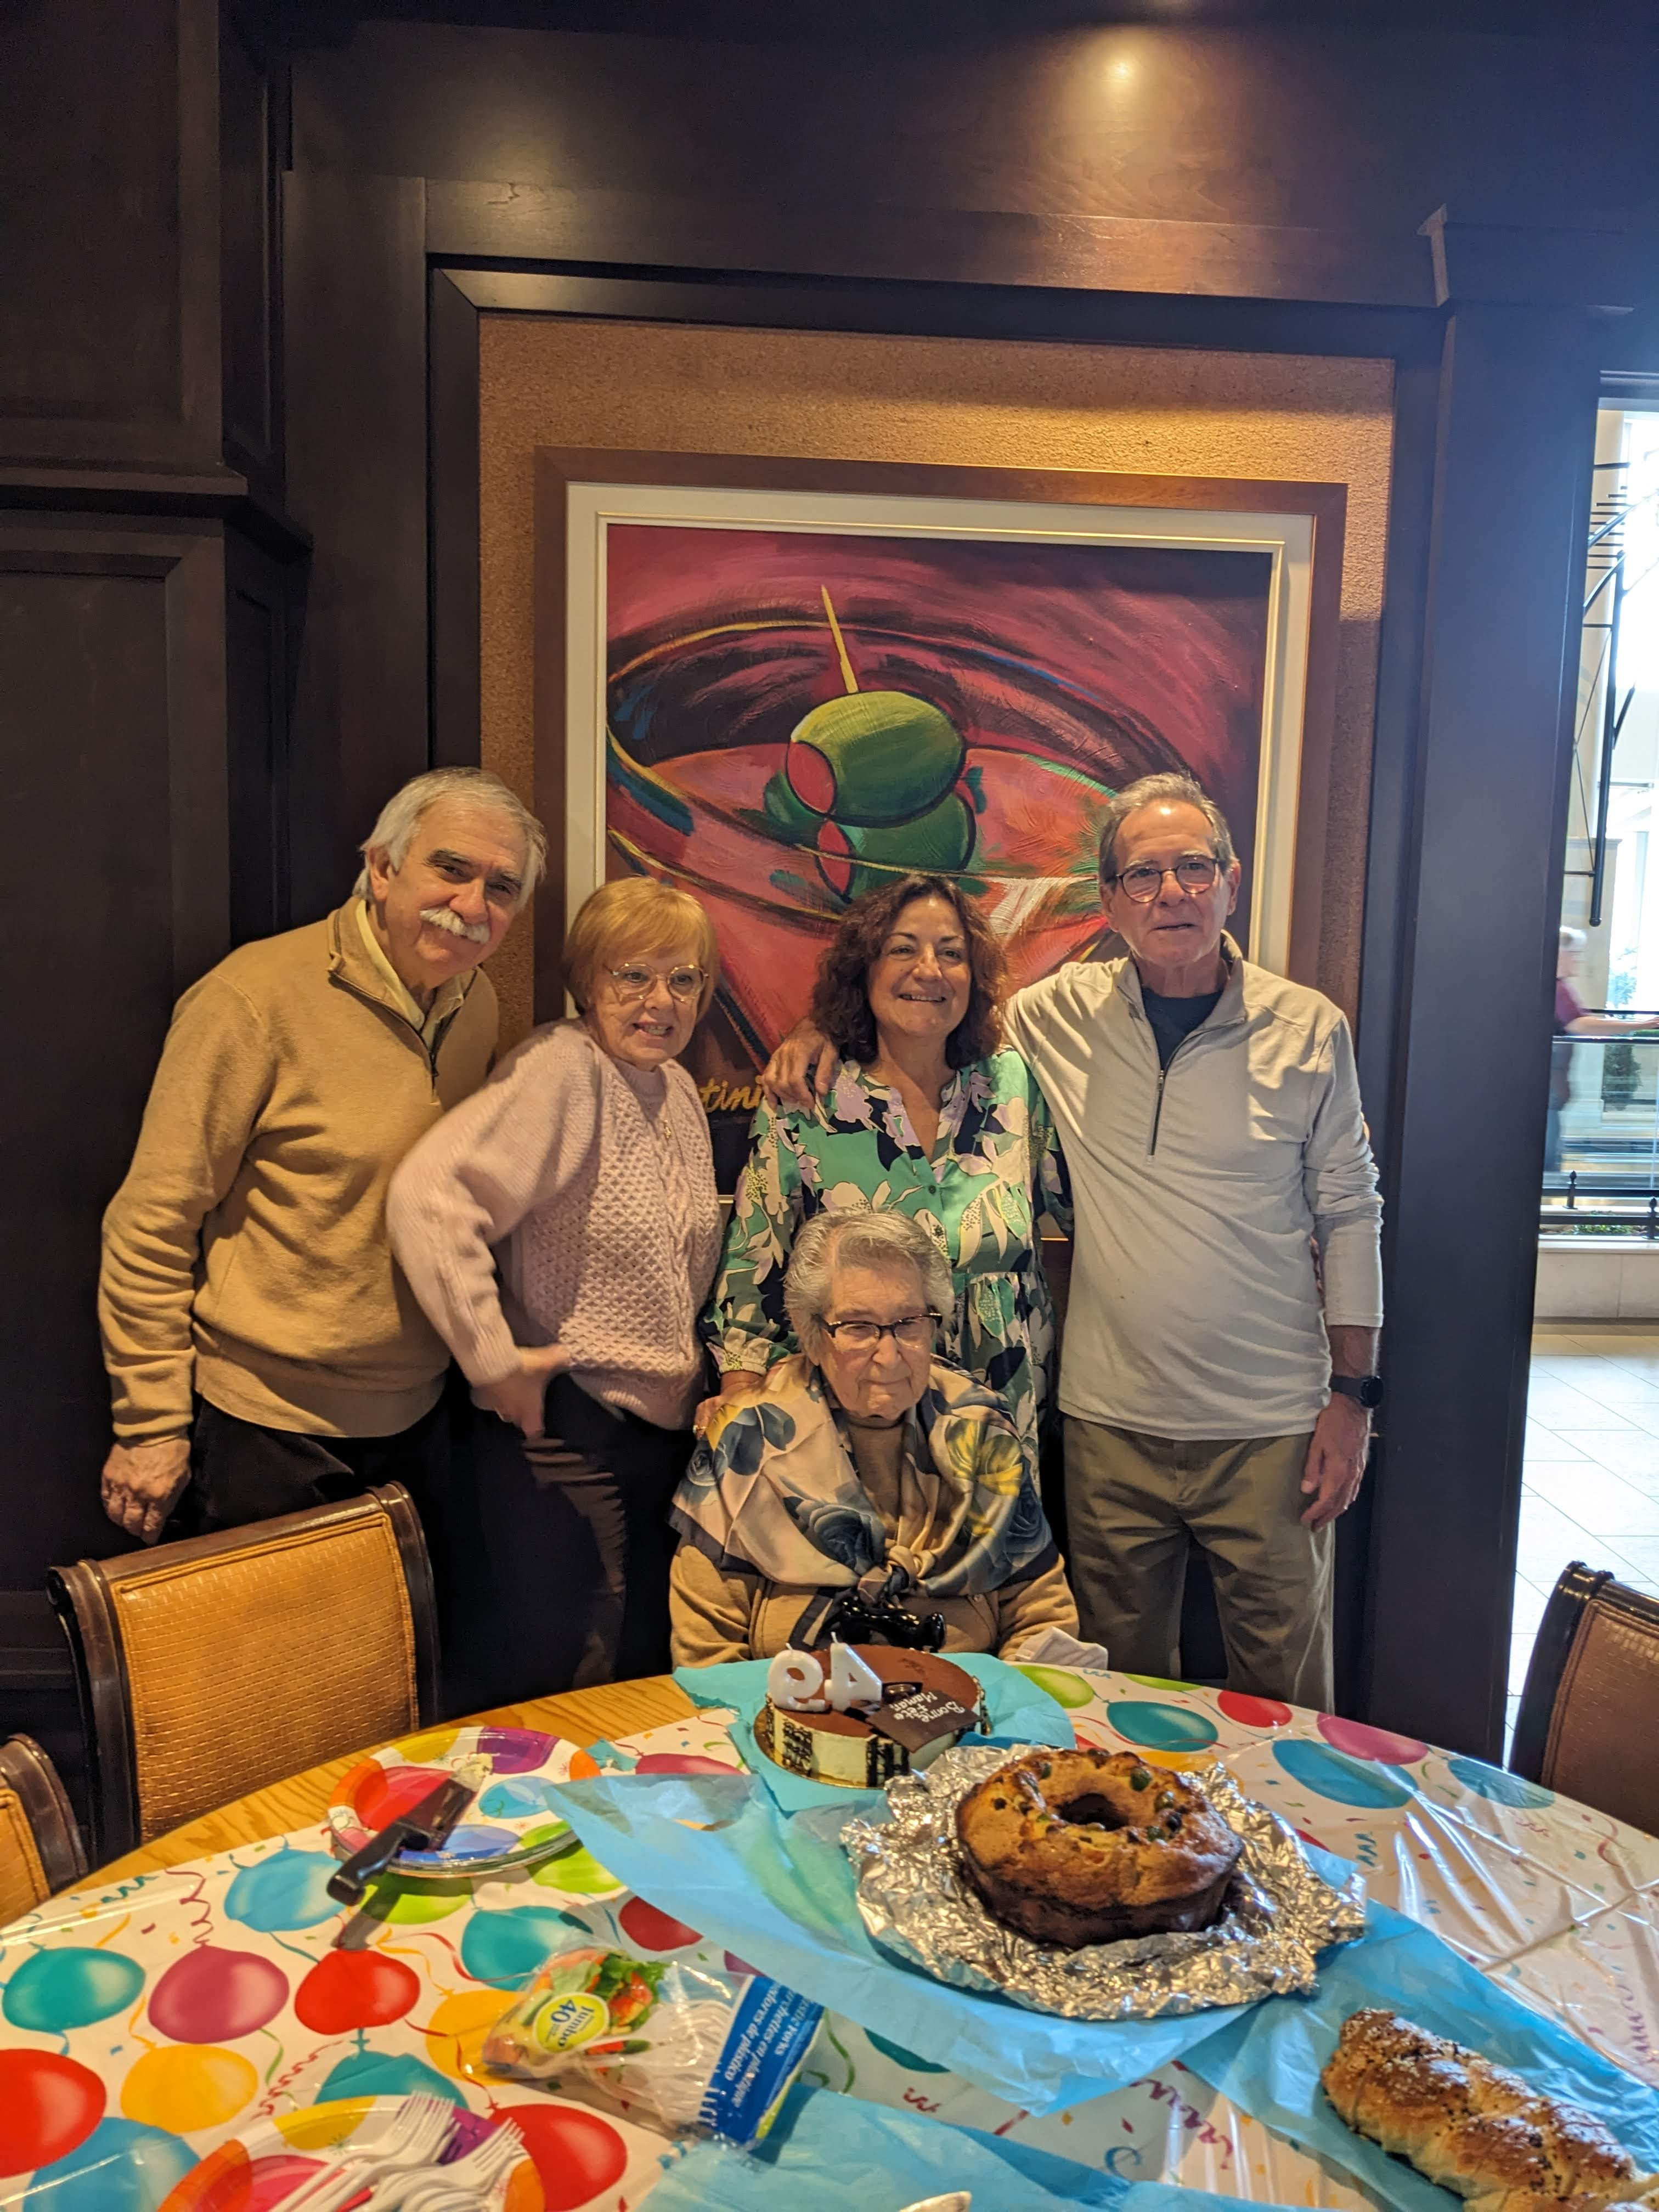
\includegraphics[width=70mm]{dermardiros/images/Ciambalone.jpg}
    \caption{Grandma Lucie's birthday in 2024}
\end{figure}
